\documentclass[a4paper,11pt]{article}
\usepackage[utf8]{inputenc}
\usepackage[MeX]{polski}
\usepackage{hyperref}
\usepackage{graphicx}
\usepackage{pdfpages}
\usepackage{tikz}
\usepackage{fancyvrb}
\usepackage{rotating}
\usepackage{multirow}
\usepackage{amsmath}
\usepackage{amsfonts}
\usetikzlibrary{positioning,shapes,shadows,arrows}

\author{Michał Aniserowicz \href{mailto:michalaniserowicz@gmail.com}{{\small \nolinkurl{<michalaniserowicz@gmail.com>}}} \\ Jakub Turek \href{mailto:jkbturek@gmail.com}{{\small \nolinkurl{<jkbturek@gmail.com>}}}}
\title{{\Large [SAG.A] Dokumentacja końcowa projektu} \\ Protokół MAS z~wykorzystaniem ontologii}
\date{2 czerwca 2013r.}

\begin{document}

\maketitle

\section{Temat projektu}

Tematem projektu jest implementacja protokołu wykorzystującego ontologię w~systemie wieloagentowym. W ramach projektu opracowana została symulacja ruchu drogowego w~kwadratowej sieci ulic przypominającej plan Manhattanu. Symulacja składa się z~następujących elementów:


\begin{description}
    \item[miasto] określa ilość przecznic (wielkość przestrzeni),
    \item[kodeks ruchu drogowego] definiuje zasady poruszania się na drodze,
    \item[sygnalizacja świetlna] określa pierwszeństwo na części skrzyżowań,
    \item[samochód] porusza się po mieście zgodnie z~zasadami ruchu drogowego znajdującymi się w~kodeksie.
\end{description}

Projekt obejmuje również przygotowanie graficznego interfejsu użytkownika, który pełni dwojaką funkcję:

\begin{itemize}
    \item ukazuje aktualny stan miasta w~rzucie z~góry,
    \item pozwala na dynamiczną zmianę kodeksu ruchu drogowego.
\end{itemize}

\section{Technologia}

Projekt został zaimplementowany na platformie JADE\footnote{Java Agent DEvelopment Framework - \href{http://jade.tilab.org}{jade.tilab.org}.}. Interfejs graficzny został stworzony z~użyciem natywnych bibliotek języka Java (AWT oraz Swing). Implementacja tworzona była w~środowisku Eclipse i~testowana w~systemie operacyjnym Windows 7 64-bit.

\section{Agenci}

W~systemie zdefiniowanych jest pięć typów agentów:

\begin{description}
    \item[Miasto] określa rozmiar (w~przecznicach) siatki miasta. Posiada zachowania umożliwiające sprawdzanie, w~których kierunkach można przemierzyć skrzyżowanie w~określonej lokalizacji. Zakłada się, że w~jednym systemie symulacji występuje wyłącznie jeden agent miasta.
    \item[Kodeks ruchu drogowego] określa następujące przepisy ruchu:
        \begin{itemize}
            \item stronę jezdni, którą poruszają się samochody,
            \item pierwszeństwo samochodu w~zależności od jego typu,
            \item kolor sygnalizacji świetlnej oznaczający, że można wjechać na skrzyżowanie,
            \item wzajemne pierwszeństwo samochodów w~sytuacji, gdy na skrzyżowaniu nie ma sygnalizacji świetlnej.
        \end{itemize}

        Zakłada się, że w~jednym systemie symulacji występuje wyłącznie jeden agent kodeksu ruchu drogowego.
    \item[Samochód] agent poruszający się po mieście. Posiada własną funkcję celu, która zmienia się wraz z~upływem czasu. Komunikuje się z~miastem, kodeksem ruchu drogowego, sygnalizatorami świetlnymi oraz innymi samochodami. Autonomicznie decyduje o~swoim zachowaniu, to znaczy, że powinien (ale nie musi) respektować przepisy ruchu drogowego zdefiniowane w~kodeksie. Porusza się w~dziedzinie dyskretnej (skokowo), lecz w~sposób płynny (wielostopniowe przejeżdżanie przez przecznicę). Występowanie agenta jest opcjonalne, dowolna jest liczba jego instancji w~jednym systemie.
    \item[Sygnalizator świetlny] steruje ruchem na skrzyżowaniu. Posiada dwa stany opisujące aktualny kolor (czerwony lub zielony), które ulegają cyklicznej zmianie. Reprezentuje grupę sygnalizatorów dla danego skrzyżowania (od dwóch do czterech, w~zależności od liczby przecinających się na skrzyżowaniu jezdni). Występowanie agenta jest opcjonalne, dowolna jest liczba jego instancji w~jednym systemie.
    \item[Mapa miasta] odwzorowywuje, rzutem z~góry, stan miasta w~danej chwili czasu. Komunikuje się z~samochodami oraz sygnalizatorami świetlnymi, odpytując cyklicznie stan agentów. Występowanie agenta jest opcjonalne, dowolna jest liczba jego instancji w~jednym systemie.
\end{description}

\section{Ontologia}

Wykorzystanie ontologii umożliwiło opisanie zmiennych zasad ruchu drogowego, do których stosują się samochody. Ontologia jest wykorzystywana głównie przez trzy typy agentów:

\begin{description}
    \item[Samochód] nie zna autonomicznie topologii miasta. Stosuje się do obowiązujących zasad ruchu drogowego narzuconych przez kodeks.
    \item[Miasto] posiada informację, w~których kierunkach można przejechać przez dane skrzyżowanie.
    \item[Kodeks ruchu drogowego] posiada informacje o~obowiązujących przepisach ruchu drogowego.
\end{description}

\subsection{Koncepcje}

Tabela \ref{tab:concepts} przedstawia koncepcje zdefiniowane w~ontologii ruchu drogowego.

\begin{table}[ht!]
    \centering
    \begin{tabular}{|c|c|c|c|}
        \hline
        \multirow{2}{*}{\textbf{Koncepcja}} & \multicolumn{3}{|c|}{\textbf{Parametr}} \\
        \cline{2-4}
        & \textbf{Nazwa} & \textbf{Typ} & \textbf{Dozwolone wartości} \\
        \hline
        \multirow{2}{*}{Pozycja} & Współrzędna $x$ & Integer & $[0;city\_size)$ \\
        \cline{2-4}
        & Współrzędna $y$ & Integer & $[0;city\_size)$ \\
        \hline
        \multirow{4}{*}{Kierunek} & \multirow{4}{*}{Kierunek} & \multirow{4}{*}{Integer} & $0$ (północ), \\
        &&& $1$ (wschód), \\
        &&& $2$ (południe), \\
        &&& $3$ (zachód) \\
        \hline
        \multirow{8}{*}{Samochód} & Pozycja & Pozycja & - \\
        \cline{2-4}
        & Kierunek & Kierunek & - \\
        \cline{2-4}
        & \multirow{2}{*}{Typ} & \multirow{2}{*}{Integer} & $0$ (normalny), \\
        &&& $1$ (uprzywilejowany), \\
        \cline{2-4}
        & \multirow{3}{*}{Status} & \multirow{3}{*}{Integer} & $0$ (jedzie), \\
        &&& $1$ (przed skrzyżowaniem), \\
        &&& $2$ (na skrzyżowaniu) \\
        \hline
        \multirow{9}{*}{Sygnalizacja} & Pozycja & Pozycja & - \\
        \cline{2-4}
        & Kolor światła & \multirow{2}{*}{Integer} & $0$ (czerwone), \\
        & (północ) & & $1$ (zielone) \\
        \cline{2-4}
        & Kolor światła & \multirow{2}{*}{Integer} & $0$ (czerwone), \\
        & (wschód) & & $1$ (zielone) \\
        \cline{2-4}
        & Kolor światła & \multirow{2}{*}{Integer} & $0$ (czerwone), \\
        & (południe) & & $1$ (zielone) \\
        \cline{2-4}
        & Kolor światła & \multirow{2}{*}{Integer} & $0$ (czerwone), \\
        & (zachód) & & $1$ (zielone) \\
        \cline{2-4}
        \hline
    \end{tabular}

    \caption{Koncepcje zdefiniowane w~ontologii ruchu drogowego.}
    \label{tab:concepts}
\end{table}

\subsection{Predykaty}
\label{sec:predicates}

Samochody komunikują się z~innymi agentami głównie przy użyciu predykatów. Tabela \ref{tab:predicates} przedstawia zdefiniowane w~ontologii miasta predykaty.

\begin{table}[ht!]
    \centering
    \begin{tabular}{|c|c|c|c|}
        \hline
        \multirow{3}{*}{\textbf{Predykat}} & \multicolumn{3}{|c|}{\textbf{Parametr}} \\
        \cline{2-4}
        & \multirow{2}{*}{\textbf{Nazwa}} & \multirow{2}{*}{\textbf{Typ}} & \textbf{Dozwolone} \\
        &&& \textbf{wartości} \\
        \hline
        Czy można & Pozycja skrzyżowania & Pozycja & - \\
        \cline{2-4}
        skręcić? & Kierunek & Kierunek & - \\
        \hline
        Czy można & \multirow{2}{*}{Kolor światła} & \multirow{2}{*}{Integer} & $0$ (czerwone), \\
        przejechać? &&& $1$ (zielone) \\
        \hline
        Czy jest & \multirow{2}{*}{Samochód} & \multirow{2}{*}{Samochód} & - \\
        uprzywilejowany? &&& \\
        \hline
        Czy ma & Samochód 1 & Samochód & - \\
        \cline{2-4}
        pierwszeństwo? & Samochód 2 & Samochód & \\
        \hline
        Czy jeździ & \multirow{2}{*}{Strona} & \multirow{2}{*}{Integer} & $0$ (lewa), \\
        po stronie? &&& $1$ (prawa) \\
        \hline
    \end{tabular}

    \caption{Predykaty zdefiniowane w~ontologii ruchu drogowego.}
    \label{tab:predicates}
\end{table}

W~dziedzinie predykatów, algorytm przejeżdżania przez skrzyżowanie można przedstawić następująco:

\begin{enumerate}
    \item Sprawdź, w~jakich kierunkach można pokonać skrzyżowanie. Prześlij do miasta predykat ,,czy można skręcić?'' z~niewiadomą typu kierunek, wypełniając jednocześnie pozycję skrzyżowania, przez które chcesz przejechać. Oczekuj na listę predykatów, które spełniają zadany warunek.
    \item Sprawdź, czy Twój samochód posiada bezwzględne pierwszeństwo. Prześlij do kodeksu ruchu drogowego predykat ,,czy ma pierwszeństwo?'' z~pojedynczym parametrem i~oczekuj na potwierdzenie jego prawdziwości.

        \begin{enumerate}
            \item Jeżeli predykat jest prawdziwy, wjedź na skrzyżowanie i~zakończ algorytm.
            \item Jeżeli predykat nie jest prawdziwy, kontynuuj algorytm.
        \end{enumerate}

    \item Sprawdź, czy na skrzyżowaniu znajdują się światła. Jeżeli nie, kontynuuj algorytm od kolejnego punktu. Jeżeli tak, sprawdź kolor świateł i~wyślij do kodeksu ruchu drogowego predykat ,,czy można przejechać?'' uzupełniony kolorem światła. Oczekuj na potwierdzenie spełnienia predykatu.

        \begin{enumerate}
            \item Jeżeli predykat jest prawdziwy, wjedź na skrzyżowanie i~zakończ algorytm.
            \item Jeżeli predykat nie jest prawdziwy, kontynuuj algorytm.
        \end{enumerate}

    \item Sprawdź, czy w~pobliżu skrzyżowania znajdują się inne samochody. Jeżeli nie, wjedź na skrzyżowanie i~zakończ algorytm. Jeżeli tak, dla każdego samochodu wypełnij predykat ,,czy ma pierwszeństwo?'' z~dwoma parametrami i~oczekuj na potwierdzenie jego prawdziwości.

        \begin{enumerate}
            \item Jeżeli wszystkie predykaty są fałszywe, wjedź na skrzyżowanie i~zakończ algorytm.
            \item Jeżeli chociaż jeden z~predykatów jest prawdziwy, oczekuj na przejechanie samochodu przez skrzyżowanie, a~następnie powtórz algorytm od punktu 4.
        \end{enumerate}
\end{enumerate}

\section{Protokół}

Wykorzystywany w~symulacji ruchu ulicznego protokół został przybliżony razem z~algorytmem opartym na predykatach w~sekcji \ref{sec:predicates}. Na następnej stronie przedstawiony jest jego większy fragment, który jest inicjowany ze strony samochodu przed wjazdem na skrzyżowanie.

Protokół jest w~całości oparty na ontologii. Komunikacja polega na przesyłaniu komunikatów w~postaci predykatów i~oczekiwaniu na odpowiedź. Na diagramie widoczne są dwa różne scenariusze wymiany informacji:

\begin{itemize}
    \item Przesłanie wypełnionego predykatu z~akcją \verb+QUERY_IF+. Oczekujemy na odpowiedź typu \verb+INFORM_IF+, która zawiera wartość logiczną, będącą odpowiedzią na pytanie czy dany predykat jest prawdziwy, czy też nie. Scenariusz ten wykorzystywany jest przy odpytywaniu kodeksu drogowego o~reguły dotyczące pierwszeństwa, wynikające z~typu samochodu, statusu sygnalizacji świetlnej lub względnej pozycji dwóch samochodów.
    \item Przesłanie częściowo wypełnionego predykatu, z~określonym polem zmiennej, z~akcją \verb+QUERY_REF+. Oczekujemy na odpowiedź, która zawiera predykat (lub listę predykatów) spełniający warunek zadany przez częściowo wypełnioną informację. Oczekiwana odpowiedź jest typu \verb+INFORM_REF+.
\end{itemize}

Diagram nie uwzględnia komunikacji pomiędzy mapą oraz innymi agentami (odpytywanie o~stan), a~także fragmentu komunikacji pomiędzy samochodem i~kodeksem ruchu drogowego dotyczącej informacji, którą stroną ulicy powinien poruszać się pojazd.

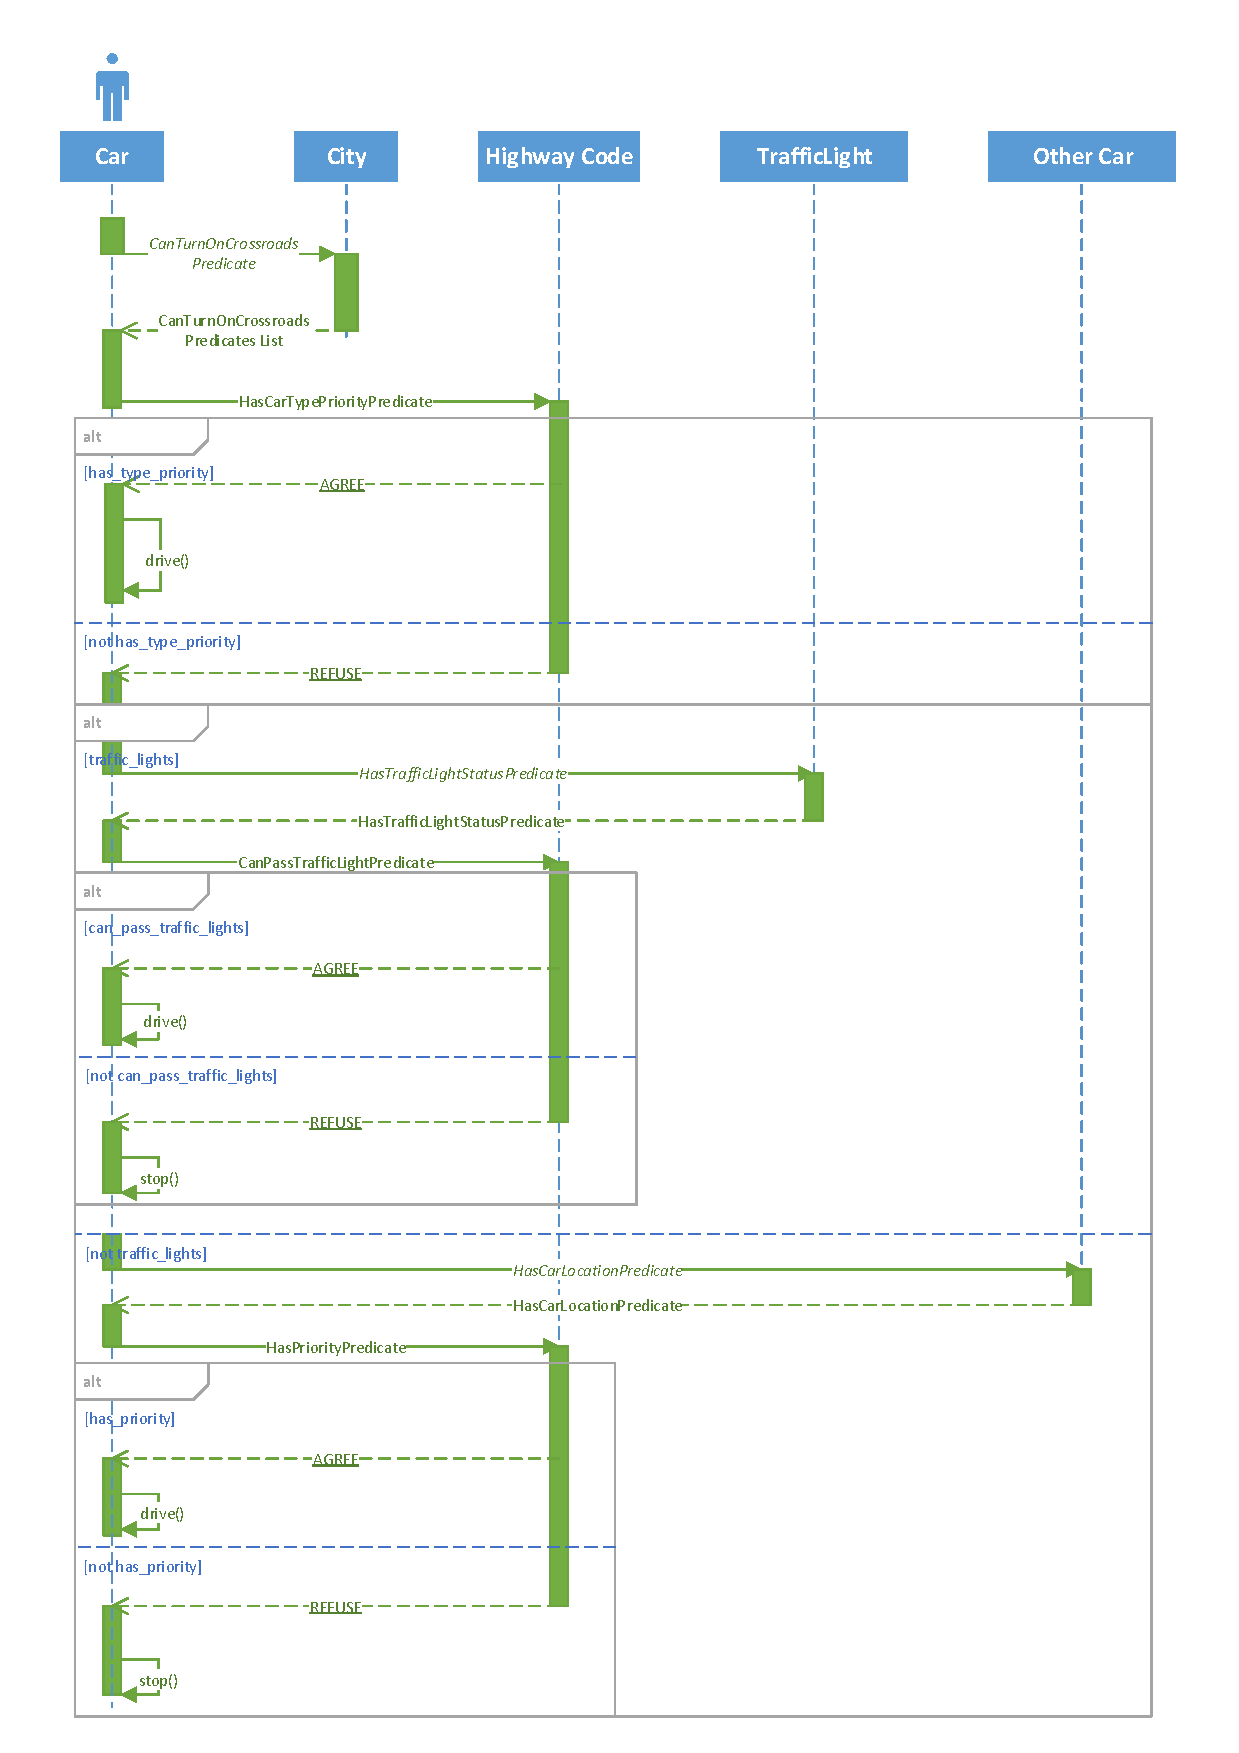
\includepdf{protocol.pdf}

\section{Parametry startowe agentów}

W~celu uruchomienia agentów należy podać właściwe im parametry startowe. W~tabeli \ref{tab:parameters} zostało zaprezentowane ich zestawienie.

\begin{table}[ht!]
    \centering
    \begin{tabular}{|c|c|c|c|c|}
        \hline
        \multirow{3}{*}{\textbf{Agent}} & \multicolumn{4}{|c|}{\textbf{Parametr}} \\
        \cline{2-5}
        & \multirow{2}{*}{\textbf{Nazwa}} & \multirow{2}{*}{\textbf{Typ}} & \textbf{Dozwolone} & \multirow{2}{*}{\textbf{Wymagalność}} \\
        &&& \textbf{wartości} & \\
        \hline
        \multirow{12}{*}{Samochód} & Pozycja $x$ & Integer & $[0;city\_size)$ & Tak \\
        \cline{2-5}
        & Pozycja $y$ & Integer & $[0;city\_size)$ & Tak \\
        \cline{2-5}
        & Prędkość & Integer & $[0;\infty)$ & Tak \\
        \cline{2-5}
        & \multirow{4}{*}{Kierunek} & \multirow{4}{*}{String} & NORTH, & \multirow{4}{*}{Tak} \\
        &&& EAST, & \\
        &&& SOUTH, & \\
        &&& WEST & \\
        \cline{2-5}
        & \multirow{3}{*}{Typ} & \multirow{3}{*}{String} & STANDARD, & \multirow{3}{*}{Tak} \\
        &&& POLICE, & \\
        &&& AMBULANCE & \\
        \cline{2-5}
        & \multirow{2}{*}{Kolor} & \multirow{2}{*}{String} & Nazwy pól & \multirow{2}{*}{Nie} \\
        &&& \href{http://docs.oracle.com/javase/1.4.2/docs/api/java/awt/Color.html}{\texttt{java.awt.Color}} & \\
        \hline
        \multirow{4}{*}{Sygnalizacja} & Pozycja $x$ & Integer & $[0;city\_size)$ & Tak \\
        \cline{2-5}
        & Pozycja $y$ & Integer & $[0;city\_size)$ & Tak \\
        \cline{2-5}
        & Częstość & \multirow{2}{*}{Integer} & \multirow{2}{*}{$[0;\infty)$} & \multirow{2}{*}{Tak} \\
        & zmiany &&& \\
        \hline
        Miasto & Rozmiar & Integer & $[0;\infty)$ & Tak \\
        \hline
    \end{tabular}

    \caption{Parametry startowe agentów.}
    \label{tab:parameters}
\end{table}

Parametry startowe należy oddzielić od siebie przecinkami. Wymagane parametry należy podać w~trakcie dołączania agenta do systemu (zarówno przez graficzny interfejs lub z~poziomu konsoli). W~przeciwnym razie rzucony zostanie wyjątek \verb+InvalidAgentArgumentsException+.

\section{Graficzny interfejs użytkownika}

Dwóch spośród wszystkich agentów zaimplementowanych w~symulatorze posiada dedykowany interfejs graficzny, który ułatwia korzystanie z~systemu:

\begin{description}
    \item[Mapa] Prezentuje stan agentów z~perspektywy rzutu prostopadłego z~nad miasta. Przykładowy widok interfejsu przedstawiony jest na rysunku \ref{img:map}. Różnokolorowe kropki znajdujące się na jezdni symbolizują samochody. Każdy samochód porusza się po odpowiednim pasie ruchu\footnote{W~przykładzie prezentowany jest ruch prawostronny, co oznacza, że samochody pomarańczowy oraz niebieski poruszają się w~kierunku północnym, natomiast biały i~czerwony - południowym.}. Sygnalizatory świetlne przedstawione są jako kropki ustawione tuż przed skrzyżowaniem, po stronie naturalnej dla wybranego typu ruchu\footnote{W~przypadku ruchu prawostronnego po prawej stronie jezdni, w~ruchu lewostronnym - po lewej.}. Oznacza to, że dla przedstawionej na rysunku sytuacji (ruch prawostronny) pomarańczowy samochód ma zielone światło. Mapa przedstawia wierne odwzorowanie stanu obiektów, utworzone na podstawie informacji zwrotnej otrzymanej od tych obiektów. Oznacza to skokowy, proporcjonalny do ustawionej przez parametry startowe prędkości, ruch każdego pojazdu.
\begin{figure}[ht!]
    \centering
    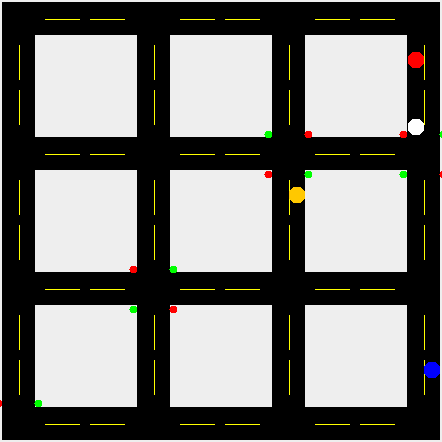
\includegraphics[width=.95\textwidth]{gui_map.png}
    \caption{Graficzny interfejs użytkownika - widok mapy.}
    \label{img:map}
\end{figure}

    \item[Kodeks ruchu drogowego] Posiada prosty interfejs graficzny, na który składa się formularz posiadający jedno pole - rozwijaną listę dostępnych w~symulacji kodeksów ruchu drogowego. Umożliwia przełączanie pomiędzy kodeksami w~czasie działania programu. Wygląd formularza przedstawia rysunek \ref{img:highway_code_selector}.
\end{description}

\begin{figure}[ht!]
    \centering
    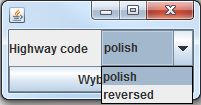
\includegraphics{gui_highway_code_selector.png}
    \caption{Graficzny interfejs użytkownika - wybór kodeksu ruchu drogowego.}
    \label{img:highway_code_selector}
\end{figure}

\section{Wnioski}

Wykorzystanie protokołu korzystającego z~ontologii w~środowisku wieloagentowym umożliwiło wierną symulację ruchu drogowego:

\begin{itemize}
    \item Zebranie zasad komunikacji określonych ściśle w~postaci protokołu pozwoliło na zwiększenie autonomiczności poszczególnych agentów:
        \begin{itemize}
            \item Samochody poruszające się w~mieście nie znają jego topologii, co pozwala na wykorzystanie ich również w~innej strukturze miasta.
            \item Mapa miasta nie przechowuje informacji o~jego stanie. W~dowolnej chwili wiernie odwzorowuje stan innych agentów.
        \end{itemize}
    \item Użycie w~protokole spójnej ontologii, opisującej dziedzinę ruchu drogowego, pozwala na:
        \begin{itemize}
            \item Realizację kodeksu ruchu drogowego a, jako konsekwencję, dynamiczną zmianę interpretacji przepisów ruchu drogowego w~czasie działania systemu.
            \item Łatwe dodawanie nieuwzględnionych przepisów ruchu drogowego, poprzez stworzenie nowych predykatów oraz reguł ich ewaluacji. Kolejne predykaty nie interferują z~poprzednio zdefiniowanymi regułami ruchu.
        \end{itemize}
\end{itemize}

Ontologia może być w~pełny sposób opisana przy pomocy klas, na które składają się wyłącznie właściwości\footnote{Dla języka Java stosowany jest termin ,,javabeans''.}. W~przypadku wykorzystania agentów osadzonych w~jednolitym środowisku opartym o~obiektowy język programowania (takim jak JADE), wygodnie jest realizować ontologię przy pomocy mechanizmu serializacji obiektów. Redukuje to narzut pracy związany z~konwertowaniem obiektów do zewnętrznego języka opisującego ontologię w~uniwersalnej gramatyce. W~ramach projektu zbadana została możliwość wykorzystania pełnej gramatyki SL\footnote{\href{http://www.fipa.org/specs/fipa00008/SC00008I.html}{FIPA SL Content Language Specification}.}.

\end{document} 